%-------------------------------------------------------------------------
\documentclass[11pt,a4paper]{article}
%-------------------------------------------------------------------------

%-------------------------------------------------------------------------
\input{corriges-ds-info-S1-preambule.tex}
%-------------------------------------------------------------------------

%-------------------------------------------------------------------------
\begin{document}
%-------------------------------------------------------------------------

$$\mbox{\textbf{\large Graphes de fonctions}}$$

\paragraph{Questions :} 
Ecrire une alternative multiple qui permette
de déterminer $y = f(x)$ pour une fonction $f$ définie par son graphe
sur $[-5;5]$ et $\forall x < -5, f(x) = f(-5)$
et $\forall x > 5, f(x) = f(5)$.

\paragraph{Réponses :} 


\begin{enumerate}

%1
\item \begin{minipage}{6.75cm}
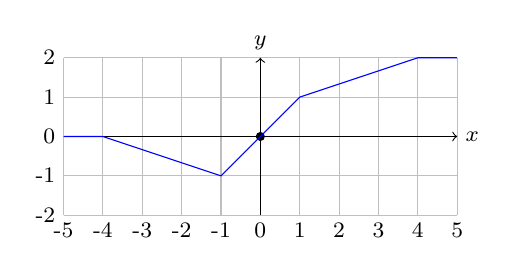
\begin{tikzpicture}[scale=0.5]\footnotesize
\draw[color=lightgray](-5,-2) grid[xstep=1,ystep=1] (5,2);
\foreach \x in {-5,-4,...,5} \draw(\x,-2) node[below]{\x};
\foreach \y in {-2,-1,...,2} \draw(-5,\y) node[left]{\y};
\filldraw(0,0) circle (0.1);
\draw[->] (-5,0) -- (5,0);
\draw (5,0) node[right]{$x$} ;
\draw[->] (0,-2) -- (0,2);
\draw (0,2) node[above]{$y$};
\draw[color=blue] (-5,0) -- (-4,0) -- (-1,-1) -- (1,1) -- (4,2) -- (5,2);
\end{tikzpicture}
\end{minipage}
\hfill
\begin{minipage}{7cm}\footnotesize
\begin{Verbatim}
if   x < -4 : y = 0
elif x < -1 : y = -x/3 - 4/3
elif x <  1 : y = x
elif x <  4 : y = x/3 + 2/3
else        : y = 2
\end{Verbatim}
\end{minipage}

%2
\item \begin{minipage}{6.75cm}
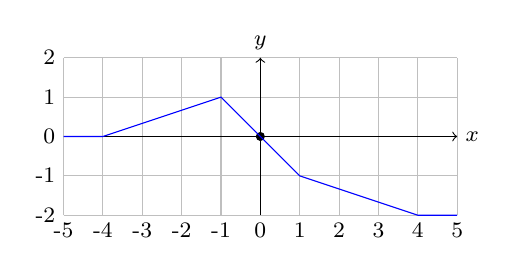
\begin{tikzpicture}[scale=0.5]\footnotesize
\draw[color=lightgray](-5,-2) grid[xstep=1,ystep=1] (5,2);
\foreach \x in {-5,-4,...,5} \draw(\x,-2) node[below]{\x};
\foreach \y in {-2,-1,...,2} \draw(-5,\y) node[left]{\y};
\filldraw(0,0) circle (0.1);
\draw[->] (-5,0) -- (5,0); 
\draw (5,0) node[right]{$x$} ;
\draw[->] (0,-2) -- (0,2);
\draw (0,2) node[above]{$y$};
\draw[color=blue] (-5,0) -- (-4,0) -- (-1,1) -- (1,-1) -- (4,-2) -- (5,-2);
\end{tikzpicture}
\end{minipage}
\hfill
\begin{minipage}{7cm}\footnotesize
\begin{Verbatim}
if   x < -4 : y = 0
elif x < -1 : y = x/3 + 4/3
elif x <  1 : y = -x
elif x <  4 : y = -x/3 - 2/3
else        : y = -2
\end{Verbatim}
\end{minipage}

%3
\item \begin{minipage}{6.75cm}
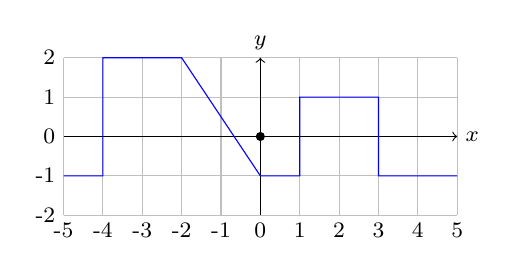
\begin{tikzpicture}[scale=0.5]\footnotesize
\draw[color=lightgray](-5,-2) grid[xstep=1,ystep=1] (5,2);
\foreach \x in {-5,-4,...,5} \draw(\x,-2) node[below]{\x};
\foreach \y in {-2,-1,...,2} \draw(-5,\y) node[left]{\y};
\filldraw(0,0) circle (0.1);
\draw[->] (-5,0) -- (5,0);
\draw (5,0) node[right]{$x$} ;
\draw[->] (0,-2) -- (0,2);
\draw (0,2) node[above]{$y$};
\draw[color=blue] (-5,-1) -- (-4,-1) -- (-4,2) -- (-2,2) -- (0,-1) -- (1,-1) -- (1,1) -- (3,1) -- (3,-1) -- (5,-1);
\end{tikzpicture}
\end{minipage}
\hfill
\begin{minipage}{7cm}\footnotesize
\begin{Verbatim}
if   x < -4 : y = -1
elif x < -2 : y = 2
elif x <  0 : y = -3*x/2 - 1
elif x <  1 : y = -1
elif x <  3 : y = 1
else        : y = -1
\end{Verbatim}
\end{minipage}

%4
\item \begin{minipage}{6.75cm}
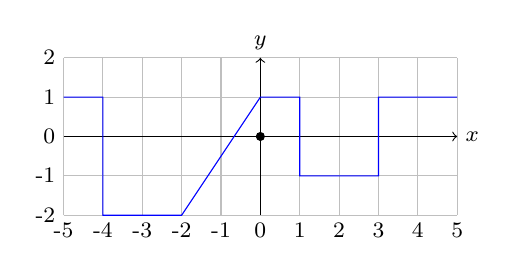
\begin{tikzpicture}[scale=0.5]\footnotesize
\draw[color=lightgray](-5,-2) grid[xstep=1,ystep=1] (5,2);
\foreach \x in {-5,-4,...,5} \draw(\x,-2) node[below]{\x};
\foreach \y in {-2,-1,...,2} \draw(-5,\y) node[left]{\y};
\filldraw(0,0) circle (0.1);
\draw[->] (-5,0) -- (5,0); 
\draw (5,0) node[right]{$x$} ;
\draw[->] (0,-2) -- (0,2);
\draw (0,2) node[above]{$y$};
\draw[color=blue] (-5,1) -- (-4,1) -- (-4,-2) -- (-2,-2) -- (0,1) -- (1,1) -- (1,-1) -- (3,-1) -- (3,1) -- (5,1);
\end{tikzpicture}
\end{minipage}
\hfill
\begin{minipage}{7cm}\footnotesize
\begin{Verbatim}
if   x < -4 : y = 1
elif x < -2 : y = -2
elif x <  0 : y = 3*x/2 + 1
elif x <  1 : y = 1
elif x <  3 : y = -1
else        : y = 1
\end{Verbatim}
\end{minipage}

%5
\item \begin{minipage}{6.75cm}
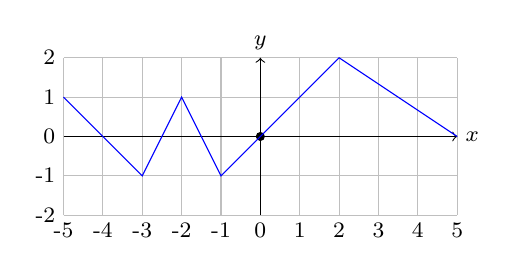
\begin{tikzpicture}[scale=0.5]\footnotesize
\draw[color=lightgray](-5,-2) grid[xstep=1,ystep=1] (5,2);
\foreach \x in {-5,-4,...,5} \draw(\x,-2) node[below]{\x};
\foreach \y in {-2,-1,...,2} \draw(-5,\y) node[left]{\y};
\filldraw(0,0) circle (0.1);
\draw[->] (-5,0) -- (5,0);
\draw (5,0) node[right]{$x$} ;
\draw[->] (0,-2) -- (0,2);
\draw (0,2) node[above]{$y$};
\draw[color=blue] (-5,1) -- (-3,-1) -- (-2,1) -- (-1,-1) -- (2,2) -- (5,0);
\end{tikzpicture}
\end{minipage}
\hfill
\begin{minipage}{7cm}\footnotesize
\begin{Verbatim}
if   x < -5 : y = 1
elif x < -3 : y = -x - 4
elif x < -2 : y = 2*x + 5
elif x < -1 : y = -2*x - 3
elif x <  2 : y = x
elif x <  5 : y = -2*x/3 + 10/3
else        : y = 0
\end{Verbatim}
\end{minipage}

%6
\item \begin{minipage}{6.75cm}
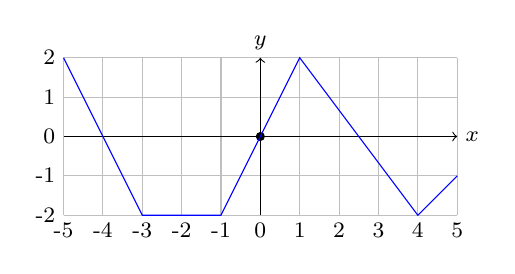
\begin{tikzpicture}[scale=0.5]\footnotesize
\draw[color=lightgray](-5,-2) grid[xstep=1,ystep=1] (5,2);
\foreach \x in {-5,-4,...,5} \draw(\x,-2) node[below]{\x};
\foreach \y in {-2,-1,...,2} \draw(-5,\y) node[left]{\y};
\filldraw(0,0) circle (0.1);
\draw[->] (-5,0) -- (5,0); 
\draw (5,0) node[right]{$x$} ;
\draw[->] (0,-2) -- (0,2);
\draw (0,2) node[above]{$y$};
\draw[color=blue] (-5,2) -- (-3,-2) -- (-1,-2) -- (1,2) -- (4,-2) -- (5,-1);
\end{tikzpicture}
\end{minipage}
\hfill
\begin{minipage}{7cm}\footnotesize
\begin{Verbatim}
if   x < -5 : y = 2
elif x < -3 : y = -2*x - 8
elif x < -1 : y = -2
elif x <  1 : y = 2*x
elif x <  4 : y = -4*x/3 + 10/3
elif x <  5 : y = x - 6
else        : y = -1
\end{Verbatim}
\end{minipage}

%7
\item \begin{minipage}{6.75cm}
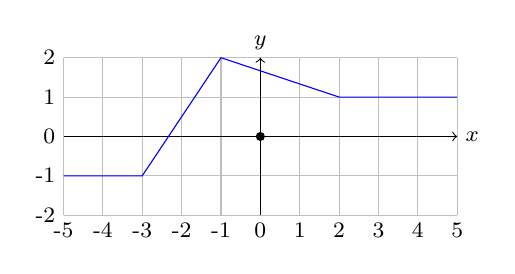
\begin{tikzpicture}[scale=0.5]\footnotesize
\draw[color=lightgray](-5,-2) grid[xstep=1,ystep=1] (5,2);
\foreach \x in {-5,-4,...,5} \draw(\x,-2) node[below]{\x};
\foreach \y in {-2,-1,...,2} \draw(-5,\y) node[left]{\y};
\filldraw(0,0) circle (0.1);
\draw[->] (-5,0) -- (5,0);
\draw (5,0) node[right]{$x$} ;
\draw[->] (0,-2) -- (0,2);
\draw (0,2) node[above]{$y$};
\draw[color=blue] (-5,-1) -- (-3,-1) -- (-1,2) -- (2,1) -- (4,1) -- (5,1);
\end{tikzpicture}
\end{minipage}
\hfill
\begin{minipage}{7cm}\footnotesize
\begin{Verbatim}
if   x < -3 : y = -1
elif x < -1 : y = 3*x/2 + 7/2
elif x <  2 : y = -x/3 + 5/3
else        : y = 1
\end{Verbatim}
\end{minipage}

%8
\item \begin{minipage}{6.75cm}
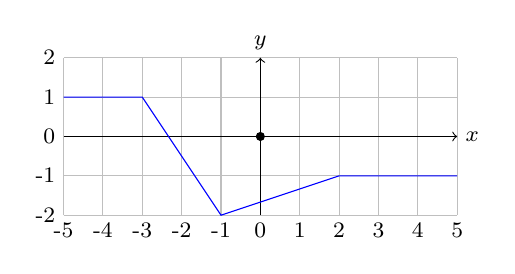
\begin{tikzpicture}[scale=0.5]\footnotesize
\draw[color=lightgray](-5,-2) grid[xstep=1,ystep=1] (5,2);
\foreach \x in {-5,-4,...,5} \draw(\x,-2) node[below]{\x};
\foreach \y in {-2,-1,...,2} \draw(-5,\y) node[left]{\y};
\filldraw(0,0) circle (0.1);
\draw[->] (-5,0) -- (5,0); 
\draw (5,0) node[right]{$x$} ;
\draw[->] (0,-2) -- (0,2);
\draw (0,2) node[above]{$y$};
\draw[color=blue] (-5,1) -- (-3,1) -- (-1,-2) -- (2,-1) -- (4,-1) -- (5,-1);
\end{tikzpicture}
\end{minipage}
\hfill
\begin{minipage}{7cm}\footnotesize
\begin{Verbatim}
if   x < -3 : y = 1
elif x < -1 : y = -3*x/2 - 7/2
elif x <  2 : y = x/3 - 5/3
else        : y = -1
\end{Verbatim}
\end{minipage}

%9
\item \begin{minipage}{6.75cm}
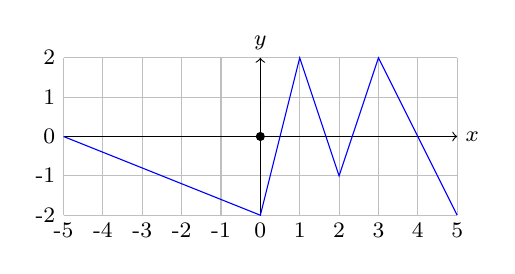
\begin{tikzpicture}[scale=0.5]\footnotesize
\draw[color=lightgray](-5,-2) grid[xstep=1,ystep=1] (5,2);
\foreach \x in {-5,-4,...,5} \draw(\x,-2) node[below]{\x};
\foreach \y in {-2,-1,...,2} \draw(-5,\y) node[left]{\y};
\filldraw(0,0) circle (0.1);
\draw[->] (-5,0) -- (5,0);
\draw (5,0) node[right]{$x$} ;
\draw[->] (0,-2) -- (0,2);
\draw (0,2) node[above]{$y$};
\draw[color=blue] (-5,0) -- (0,-2) -- (1,2) -- (2,-1) -- (3,2) -- (5,-2);
\end{tikzpicture}
\end{minipage}
\hfill
\begin{minipage}{7cm}\footnotesize
\begin{Verbatim}
if   x < -5 : y = 0
elif x <  0 : y = -2*x/5 - 2
elif x <  1 : y = 4*x - 2
elif x <  2 : y = -3*x + 5
elif x <  3 : y = 3*x - 7
elif x <  5 : y = -2*x + 8
else        : y = -2
\end{Verbatim}
\end{minipage}

%10
\item \begin{minipage}{6.75cm}
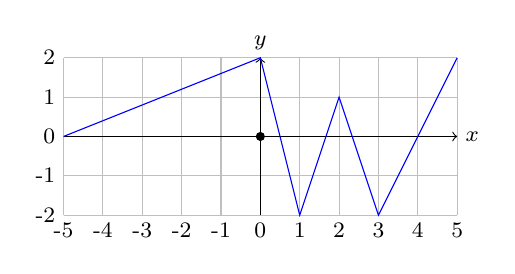
\begin{tikzpicture}[scale=0.5]\footnotesize
\draw[color=lightgray](-5,-2) grid[xstep=1,ystep=1] (5,2);
\foreach \x in {-5,-4,...,5} \draw(\x,-2) node[below]{\x};
\foreach \y in {-2,-1,...,2} \draw(-5,\y) node[left]{\y};
\filldraw(0,0) circle (0.1);
\draw[->] (-5,0) -- (5,0); 
\draw (5,0) node[right]{$x$} ;
\draw[->] (0,-2) -- (0,2);
\draw (0,2) node[above]{$y$};
\draw[color=blue] (-5,0) -- (0,2) -- (1,-2) -- (2,1) -- (3,-2) -- (5,2);
\end{tikzpicture}
\end{minipage}
\hfill
\begin{minipage}{7cm}\footnotesize
\begin{Verbatim}
if   x < -5 : y = 0
elif x <  0 : y = 2*x/5 + 2
elif x <  1 : y = -4*x + 2
elif x <  2 : y = 3*x - 5
elif x <  3 : y = -3*x + 7
elif x <  5 : y = 2*x - 8
else        : y = 2
\end{Verbatim}
\end{minipage}

%11
\item \begin{minipage}{6.75cm}
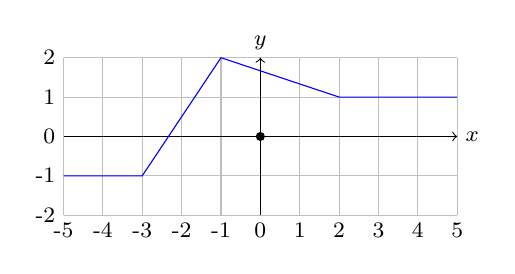
\begin{tikzpicture}[scale=0.5]\footnotesize
\draw[color=lightgray](-5,-2) grid[xstep=1,ystep=1] (5,2);
\foreach \x in {-5,-4,...,5} \draw(\x,-2) node[below]{\x};
\foreach \y in {-2,-1,...,2} \draw(-5,\y) node[left]{\y};
\filldraw(0,0) circle (0.1);
\draw[->] (-5,0) -- (5,0);
\draw (5,0) node[right]{$x$} ;
\draw[->] (0,-2) -- (0,2);
\draw (0,2) node[above]{$y$};
\draw[color=blue] (-5,-1) -- (-3,-1) -- (-1,2) -- (2,1) -- (4,1) -- (5,1);
\end{tikzpicture}
\end{minipage}
\hfill
\begin{minipage}{7cm}\footnotesize
\begin{Verbatim}
if   x < -3 : y = -1
elif x < -1 : y = 3*x/2 + 7/2
elif x <  2 : y = -x/3 + 5/3
else        : y = 1
\end{Verbatim}
\end{minipage}

%12
\item \begin{minipage}{6.75cm}
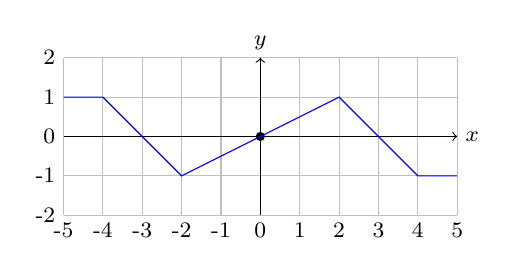
\begin{tikzpicture}[scale=0.5]\footnotesize
\draw[color=lightgray](-5,-2) grid[xstep=1,ystep=1] (5,2);
\foreach \x in {-5,-4,...,5} \draw(\x,-2) node[below]{\x};
\foreach \y in {-2,-1,...,2} \draw(-5,\y) node[left]{\y};
\filldraw(0,0) circle (0.1);
\draw[->] (-5,0) -- (5,0);
\draw (5,0) node[right]{$x$} ;
\draw[->] (0,-2) -- (0,2);
\draw (0,2) node[above]{$y$};
\draw[color=blue] (-5,1) -- (-4,1) -- (-2,-1) -- (2,1) -- (4,-1) -- (5,-1);
\end{tikzpicture}
\end{minipage}
\hfill
\begin{minipage}{7cm}\footnotesize
\begin{Verbatim}
if   x < -4 : y = 1
elif x < -2 : y = -x - 3
elif x <  2 : y = x/2
elif x <  4 : y = -x + 3
else        : y = -1
\end{Verbatim}
\end{minipage}

%13
\item \begin{minipage}{6.75cm}
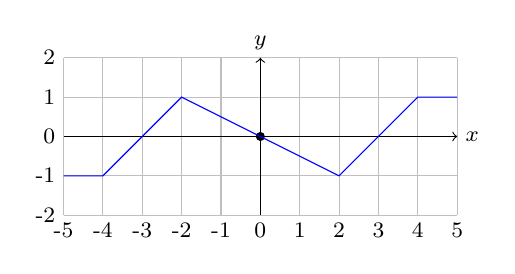
\begin{tikzpicture}[scale=0.5]\footnotesize
\draw[color=lightgray](-5,-2) grid[xstep=1,ystep=1] (5,2);
\foreach \x in {-5,-4,...,5} \draw(\x,-2) node[below]{\x};
\foreach \y in {-2,-1,...,2} \draw(-5,\y) node[left]{\y};
\filldraw(0,0) circle (0.1);
\draw[->] (-5,0) -- (5,0); 
\draw (5,0) node[right]{$x$} ;
\draw[->] (0,-2) -- (0,2);
\draw (0,2) node[above]{$y$};
\draw[color=blue] (-5,-1) -- (-4,-1) -- (-2,1) -- (2,-1) -- (4,1) -- (5,1);
\end{tikzpicture}
\end{minipage}
\hfill
\begin{minipage}{7cm}\footnotesize
\begin{Verbatim}
if   x < -4 : y = -1
elif x < -2 : y = x + 3
elif x <  2 : y = -x/2
elif x <  4 : y = x - 3
else        : y = 1
\end{Verbatim}
\end{minipage}

%14
\item \begin{minipage}{6.75cm}
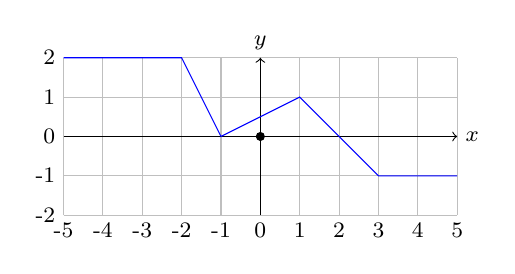
\begin{tikzpicture}[scale=0.5]\footnotesize
\draw[color=lightgray](-5,-2) grid[xstep=1,ystep=1] (5,2);
\foreach \x in {-5,-4,...,5} \draw(\x,-2) node[below]{\x};
\foreach \y in {-2,-1,...,2} \draw(-5,\y) node[left]{\y};
\filldraw(0,0) circle (0.1);
\draw[->] (-5,0) -- (5,0);
\draw (5,0) node[right]{$x$} ;
\draw[->] (0,-2) -- (0,2);
\draw (0,2) node[above]{$y$};
\draw[color=blue] (-5,2) -- (-2,2) -- (-1,0) -- (1,1) -- (3,-1) -- (5,-1);
\end{tikzpicture}
\end{minipage}
\hfill
\begin{minipage}{7cm}\footnotesize
\begin{Verbatim}
if   x < -2 : y = 2
elif x < -1 : y = -2*x - 2
elif x <  1 : y = x/2 + 1/2
elif x <  3 : y = -x + 2
else        : y = -1
\end{Verbatim}
\end{minipage}

%15
\item \begin{minipage}{6.75cm}
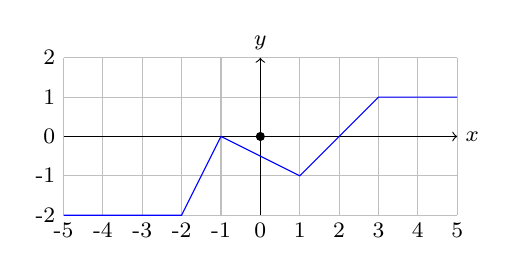
\begin{tikzpicture}[scale=0.5]\footnotesize
\draw[color=lightgray](-5,-2) grid[xstep=1,ystep=1] (5,2);
\foreach \x in {-5,-4,...,5} \draw(\x,-2) node[below]{\x};
\foreach \y in {-2,-1,...,2} \draw(-5,\y) node[left]{\y};
\filldraw(0,0) circle (0.1);
\draw[->] (-5,0) -- (5,0); 
\draw (5,0) node[right]{$x$} ;
\draw[->] (0,-2) -- (0,2);
\draw (0,2) node[above]{$y$};
\draw[color=blue] (-5,-2) -- (-2,-2) -- (-1,0) -- (1,-1) -- (3,1) -- (5,1);
\end{tikzpicture}
\end{minipage}
\hfill
\begin{minipage}{7cm}\footnotesize
\begin{Verbatim}
if   x < -2 : y = -2
elif x < -1 : y = 2*x + 2
elif x <  1 : y = -x/2 - 1/2
elif x <  3 : y = x - 2
else        : y = 1
\end{Verbatim}
\end{minipage}

%16
\item \begin{minipage}{6.75cm}
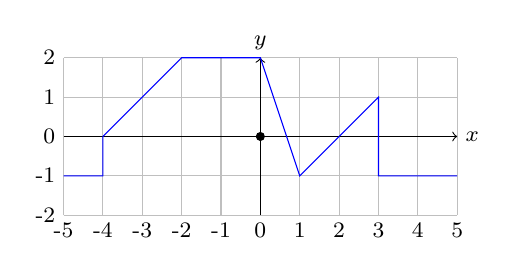
\begin{tikzpicture}[scale=0.5]\footnotesize
\draw[color=lightgray](-5,-2) grid[xstep=1,ystep=1] (5,2);
\foreach \x in {-5,-4,...,5} \draw(\x,-2) node[below]{\x};
\foreach \y in {-2,-1,...,2} \draw(-5,\y) node[left]{\y};
\filldraw(0,0) circle (0.1);
\draw[->] (-5,0) -- (5,0);
\draw (5,0) node[right]{$x$} ;
\draw[->] (0,-2) -- (0,2);
\draw (0,2) node[above]{$y$};
\draw[color=blue] (-5,-1) -- (-4,-1) -- (-4,0) -- (-2,2) -- (0,2) -- (1,-1) -- (1,-1) -- (3,1) -- (3,-1) -- (5,-1);
\end{tikzpicture}
\end{minipage}
\hfill
\begin{minipage}{7cm}\footnotesize
\begin{Verbatim}
if   x < -4 : y = -1
elif x < -2 : y = x + 4
elif x <  0 : y = 2
elif x <  1 : y = -3*x + 2
elif x <  3 : y = x - 2
else        : y = -1
\end{Verbatim}
\end{minipage}

%17
\item \begin{minipage}{6.75cm}
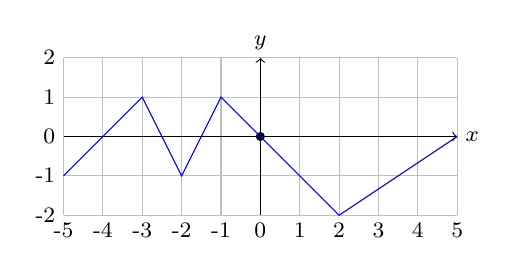
\begin{tikzpicture}[scale=0.5]\footnotesize
\draw[color=lightgray](-5,-2) grid[xstep=1,ystep=1] (5,2);
\foreach \x in {-5,-4,...,5} \draw(\x,-2) node[below]{\x};
\foreach \y in {-2,-1,...,2} \draw(-5,\y) node[left]{\y};
\filldraw(0,0) circle (0.1);
\draw[->] (-5,0) -- (5,0); 
\draw (5,0) node[right]{$x$} ;
\draw[->] (0,-2) -- (0,2);
\draw (0,2) node[above]{$y$};
\draw[color=blue] (-5,-1) -- (-3,1) -- (-2,-1) -- (-1,1) -- (2,-2) -- (5,0);
\end{tikzpicture}
\end{minipage}
\hfill
\begin{minipage}{7cm}\footnotesize
\begin{Verbatim}
if   x < -5 : y = -1
elif x < -3 : y = x + 4
elif x < -2 : y = -2*x - 5
elif x < -1 : y = 2*x + 3
elif x <  2 : y = -x
elif x <  5 : y = 2*x/3 - 10/3
else        : y = 0
\end{Verbatim}
\end{minipage}

%18
\item \begin{minipage}{6.75cm}
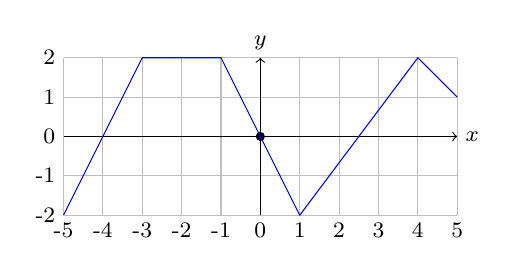
\begin{tikzpicture}[scale=0.5]\footnotesize
\draw[color=lightgray](-5,-2) grid[xstep=1,ystep=1] (5,2);
\foreach \x in {-5,-4,...,5} \draw(\x,-2) node[below]{\x};
\foreach \y in {-2,-1,...,2} \draw(-5,\y) node[left]{\y};
\filldraw(0,0) circle (0.1);
\draw[->] (-5,0) -- (5,0);
\draw (5,0) node[right]{$x$} ;
\draw[->] (0,-2) -- (0,2);
\draw (0,2) node[above]{$y$};
\draw[color=blue] (-5,-2) -- (-3,2) -- (-1,2) -- (1,-2) -- (4,2) -- (5,1);
\end{tikzpicture}
\end{minipage}
\hfill
\begin{minipage}{7cm}\footnotesize
\begin{Verbatim}
if   x < -5 : y = -2
elif x < -3 : y = 2*x + 8
elif x < -1 : y = 2
elif x <  1 : y = -2*x
elif x <  4 : y = 4*x/3 - 10/3
elif x <  5 : y = -x + 6
else        : y = 1
\end{Verbatim}
\end{minipage}

%19
\item \begin{minipage}{6.75cm}
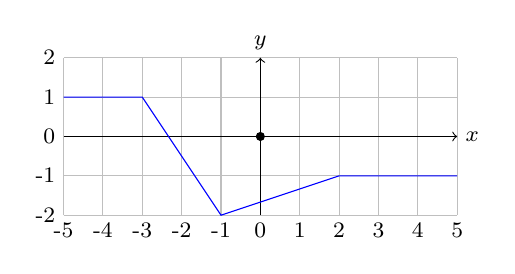
\begin{tikzpicture}[scale=0.5]\footnotesize
\draw[color=lightgray](-5,-2) grid[xstep=1,ystep=1] (5,2);
\foreach \x in {-5,-4,...,5} \draw(\x,-2) node[below]{\x};
\foreach \y in {-2,-1,...,2} \draw(-5,\y) node[left]{\y};
\filldraw(0,0) circle (0.1);
\draw[->] (-5,0) -- (5,0); 
\draw (5,0) node[right]{$x$} ;
\draw[->] (0,-2) -- (0,2);
\draw (0,2) node[above]{$y$};
\draw[color=blue] (-5,1) -- (-3,1) -- (-1,-2) -- (2,-1) -- (4,-1) -- (5,-1);
\end{tikzpicture}
\end{minipage}
\hfill
\begin{minipage}{7cm}\footnotesize
\begin{Verbatim}
if   x < -3 : y = 1
elif x < -1 : y = -3*x/2 - 7/2
elif x <  2 : y = x/3 - 5/3
else        : y = -1
\end{Verbatim}
\end{minipage}

%20
\item \begin{minipage}{6.75cm}
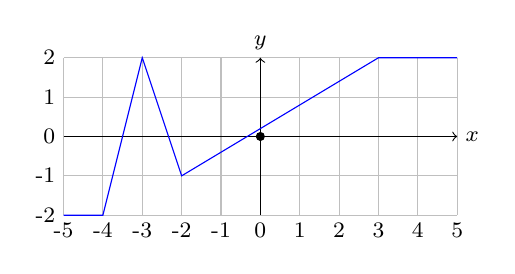
\begin{tikzpicture}[scale=0.5]\footnotesize
\draw[color=lightgray](-5,-2) grid[xstep=1,ystep=1] (5,2);
\foreach \x in {-5,-4,...,5} \draw(\x,-2) node[below]{\x};
\foreach \y in {-2,-1,...,2} \draw(-5,\y) node[left]{\y};
\filldraw(0,0) circle (0.1);
\draw[->] (-5,0) -- (5,0);
\draw (5,0) node[right]{$x$} ;
\draw[->] (0,-2) -- (0,2);
\draw (0,2) node[above]{$y$};
\draw[color=blue] (-5,-2) -- (-4,-2) -- (-3,2) -- (-2,-1) -- (3,2) -- (5,2);
\end{tikzpicture}
\end{minipage}
\hfill
\begin{minipage}{7cm}\footnotesize
\begin{Verbatim}
if   x < -4 : y = -2
elif x < -3 : y = 4*x + 14
elif x < -2 : y = -3*x - 7
elif x <  3 : y = 3*x/5 + 1/5
else        : y = 2
\end{Verbatim}
\end{minipage}

%21
\item \begin{minipage}{6.75cm}
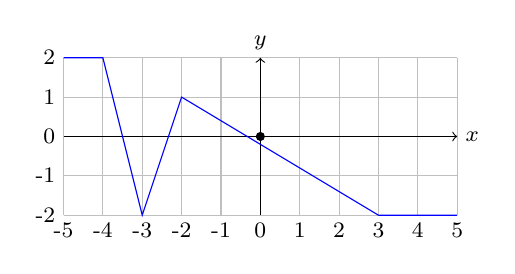
\begin{tikzpicture}[scale=0.5]\footnotesize
\draw[color=lightgray](-5,-2) grid[xstep=1,ystep=1] (5,2);
\foreach \x in {-5,-4,...,5} \draw(\x,-2) node[below]{\x};
\foreach \y in {-2,-1,...,2} \draw(-5,\y) node[left]{\y};
\filldraw(0,0) circle (0.1);
\draw[->] (-5,0) -- (5,0); 
\draw (5,0) node[right]{$x$} ;
\draw[->] (0,-2) -- (0,2);
\draw (0,2) node[above]{$y$};
\draw[color=blue] (-5,2) -- (-4,2) -- (-3,-2) -- (-2,1) -- (3,-2) -- (5,-2);
\end{tikzpicture}
\end{minipage}
\hfill
\begin{minipage}{7cm}\footnotesize
\begin{Verbatim}
if   x < -4 : y = 2
elif x < -3 : y = -4*x - 14
elif x < -2 : y = 3*x + 7
elif x <  3 : y = -3*x/5 - 1/5
else        : y = -2
\end{Verbatim}
\end{minipage}

%22
\item \begin{minipage}{6.75cm}
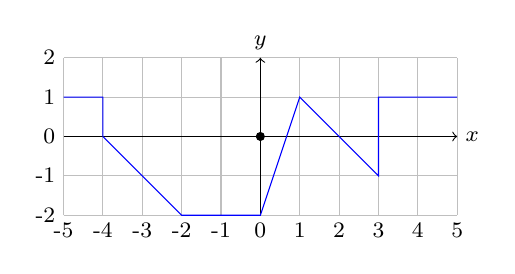
\begin{tikzpicture}[scale=0.5]\footnotesize
\draw[color=lightgray](-5,-2) grid[xstep=1,ystep=1] (5,2);
\foreach \x in {-5,-4,...,5} \draw(\x,-2) node[below]{\x};
\foreach \y in {-2,-1,...,2} \draw(-5,\y) node[left]{\y};
\filldraw(0,0) circle (0.1);
\draw[->] (-5,0) -- (5,0); 
\draw (5,0) node[right]{$x$} ;
\draw[->] (0,-2) -- (0,2);
\draw (0,2) node[above]{$y$};
\draw[color=blue] (-5,1) -- (-4,1) -- (-4,0) -- (-2,-2) -- (0,-2) -- (1,1) -- (1,1) -- (3,-1) -- (3,1) -- (5,1);
\end{tikzpicture}
\end{minipage}
\hfill
\begin{minipage}{7cm}\footnotesize
\begin{Verbatim}
if   x < -4 : y = 1
elif x < -2 : y = -x - 4
elif x <  0 : y = -2
elif x <  1 : y = 3*x - 2
elif x <  3 : y = -x + 2
else        : y = 1
\end{Verbatim}
\end{minipage}

%23
\item \begin{minipage}{6.75cm}
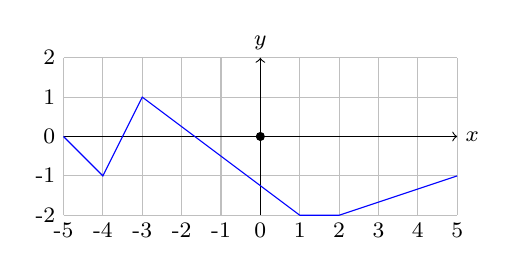
\begin{tikzpicture}[scale=0.5]\footnotesize
\draw[color=lightgray](-5,-2) grid[xstep=1,ystep=1] (5,2);
\foreach \x in {-5,-4,...,5} \draw(\x,-2) node[below]{\x};
\foreach \y in {-2,-1,...,2} \draw(-5,\y) node[left]{\y};
\filldraw(0,0) circle (0.1);
\draw[->] (-5,0) -- (5,0); 
\draw (5,0) node[right]{$x$} ;
\draw[->] (0,-2) -- (0,2);
\draw (0,2) node[above]{$y$};
\draw[color=blue] (-5,0) -- (-4,-1) -- (-3,1) -- (1,-2) -- (2,-2) -- (5,-1);
\end{tikzpicture}
\end{minipage}
\hfill
\begin{minipage}{7cm}\footnotesize
\begin{Verbatim}
if   x < -5 : y = 0
elif x < -4 : y = x + 5
elif x < -3 : y = -2*x - 7
elif x <  1 : y = -3*x/4 - 5/4
elif x <  2 : y = -2
elif x <  5 : y = x/3 - 8/3
else        : y = -1
\end{Verbatim}
\end{minipage}

%24
\item \begin{minipage}{6.75cm}
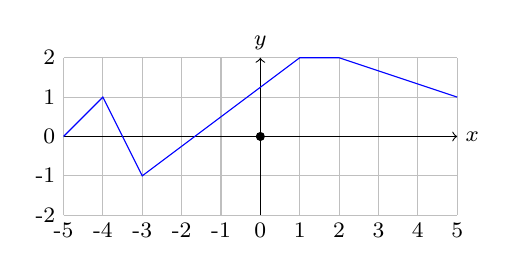
\begin{tikzpicture}[scale=0.5]\footnotesize
\draw[color=lightgray](-5,-2) grid[xstep=1,ystep=1] (5,2);
\foreach \x in {-5,-4,...,5} \draw(\x,-2) node[below]{\x};
\foreach \y in {-2,-1,...,2} \draw(-5,\y) node[left]{\y};
\filldraw(0,0) circle (0.1);
\draw[->] (-5,0) -- (5,0);
\draw (5,0) node[right]{$x$} ;
\draw[->] (0,-2) -- (0,2);
\draw (0,2) node[above]{$y$};
\draw[color=blue] (-5,0) -- (-4,1) -- (-3,-1) -- (1,2) -- (2,2) -- (5,1);
\end{tikzpicture}
\end{minipage}
\hfill
\begin{minipage}{7cm}\footnotesize
\begin{Verbatim}
if   x < -5 : y = 0
elif x < -4 : y = -x - 5
elif x < -3 : y = 2*x + 7
elif x <  1 : y = 3*x/4 + 5/4
elif x <  2 : y = 2
elif x <  5 : y = -x/3 + 8/3
else        : y = 1
\end{Verbatim}
\end{minipage}

\end{enumerate}

%-------------------------------------------------------------------------
\end{document}
%-------------------------------------------------------------------------
